% Composición de capas equivariantes
% Compilar con: pdflatex equivariant_composition.tex
\documentclass[tikz,border=10pt]{standalone}
\usepackage{tikz}
\usepackage{amsmath}
\usetikzlibrary{arrows.meta, positioning, shapes.geometric, calc}

\definecolor{gdlblue}{RGB}{41, 98, 168}
\definecolor{gdlred}{RGB}{191, 49, 49}
\definecolor{gdlgreen}{RGB}{30, 130, 76}
\definecolor{gdlorange}{RGB}{217, 130, 30}
\definecolor{gdlpurple}{RGB}{118, 56, 138}
\definecolor{gdlgray}{RGB}{140, 140, 140}
\definecolor{gdlyellow}{RGB}{190, 140, 10}

\begin{document}
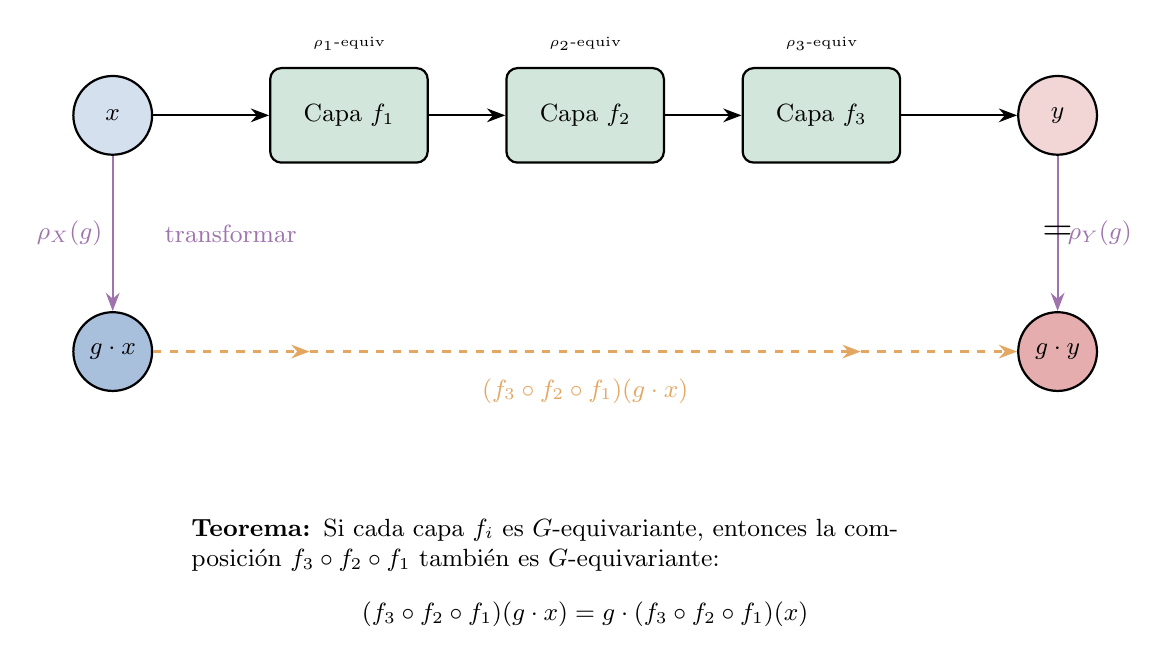
\begin{tikzpicture}[
    >=Stealth,
    layer/.style={rectangle, draw, thick, rounded corners, minimum width=2cm, minimum height=1.2cm, font=\small},
    data/.style={circle, draw, thick, minimum size=1cm, font=\small},
    arrow/.style={->, thick}
]

% === Red neuronal equivariante ===
% Datos de entrada
\node[data, fill=gdlblue!20] (x) at (0, 0) {$x$};

% Capas
\node[layer, fill=gdlgreen!20] (f1) at (3, 0) {Capa $f_1$};
\node[layer, fill=gdlgreen!20] (f2) at (6, 0) {Capa $f_2$};
\node[layer, fill=gdlgreen!20] (f3) at (9, 0) {Capa $f_3$};

% Salida
\node[data, fill=gdlred!20] (y) at (12, 0) {$y$};

% Flechas principales
\draw[arrow] (x) -- (f1);
\draw[arrow] (f1) -- (f2);
\draw[arrow] (f2) -- (f3);
\draw[arrow] (f3) -- (y);

% === Acción del grupo (fila inferior) ===
\node[data, fill=gdlblue!40] (gx) at (0, -3) {$g \cdot x$};
\node[data, fill=gdlred!40] (gy) at (12, -3) {$g \cdot y$};

% Flechas de acción del grupo
\draw[arrow, gdlpurple!70] (x) -- node[left, font=\small] {$\rho_X(g)$} (gx);
\draw[arrow, gdlpurple!70] (y) -- node[right, font=\small] {$\rho_Y(g)$} (gy);

% Camino por abajo (composición)
\draw[arrow, dashed, gdlorange!70] (gx) -- ++(2.5, 0);
\draw[arrow, dashed, gdlorange!70] (2.5, -3) -- (9.5, -3);
\draw[arrow, dashed, gdlorange!70] (9.5, -3) -- (gy);

% === Etiquetas de equivarianza ===
\node[font=\small, gdlpurple!70] at (1.5, -1.5) {transformar};
\node[font=\small, gdlorange!70] at (6, -3.5) {$(f_3 \circ f_2 \circ f_1)(g \cdot x)$};

% === Símbolo de igualdad ===
\node[font=\Large] at (12, -1.5) {$=$};

% === Teorema ===
\node[font=\small, text width=10cm, below] at (6, -5) {
    \textbf{Teorema:} Si cada capa $f_i$ es $G$-equivariante, entonces la composición $f_3 \circ f_2 \circ f_1$ también es $G$-equivariante:
    \[(f_3 \circ f_2 \circ f_1)(g \cdot x) = g \cdot (f_3 \circ f_2 \circ f_1)(x)\]
};

% === Etiquetas de representaciones intermedias ===
\node[font=\tiny, above] at (3, 0.7) {$\rho_1$-equiv};
\node[font=\tiny, above] at (6, 0.7) {$\rho_2$-equiv};
\node[font=\tiny, above] at (9, 0.7) {$\rho_3$-equiv};

\end{tikzpicture}
\end{document}
